%! Author = songshgeo
%! Date = 2022/3/10

% 现有制度匹配知识的两个特别弱点包括理解(图~\ref{fig:framework}~\textbf{b}):(i)社会经济体系结构和结果之间的因果联系;(ii)由于制度上缺乏匹配而导致的基本过程的细节,特别是不同参与者的激励。
% 这些弱点限制了对制度设计的理解,阻碍了对制度匹配的研究。

为了更好地理解自上而下的制度改革对黄河流域产生的影响,本章以黄河流域的水资源分配制度为例,重点关注两次重大制度转变:1987年提出的“八七”分水方案和1998年的提出的流域统一调度。
研究选择水资源分配制度为切入点的主要理由如下:
(1) 本章关注自上而下的制度变迁对人-水关系的影响,而黄河的水资源配额制度是典型的由中央主导的改革,利益相关者(相关各省)之间没有相互作用。
(2) 很少有大型流域经历这种制度转变一次以上,1987和1998前后两次制度变革具有难得的可对比性,提供了绝妙的准自然实验。
(3) 两次制度改革之间维持的时间周期足够长,便于对数据进行时间序列分析,且该研究时段完全覆盖了第三章中识别的“治理转型时期”。

% 为了量化制度变迁为黄河流域用水带来的影响,我们按附图1所示的技术路线执行了分析过程
本章研究重点关注上述两次水资源配额制度改革对1979年至2008年黄河流域的用水变化,两次制度变迁将这段研究时期分为均匀的三个时间序列:$1979-1987$,$1988-1998$,$1999-2008$。
我们首先详细介绍了两次制度改革的背景及特点,以及刻画其社会-生态系统结构模块的方法。
接下来收集用以构建反事实推断模型的数据集并使用主成分分析(PCA)方法对其进行降维。
最后,我们利用差分合成控制法(DSC)构建了反事实推断模型\cite{arkhangelsky2021},估算了“如果没有发生制度转变”时的用水量,从而分析两种制度变迁对黄河流域各省份用水量变化的净影响。
% 最后,在理论讨论方面,我们基于已确定的SES结构进行了边际效益分析,为观测到的用水变化模式提供了理论解释。

\subsection{制度背景介绍}\label{sec:yrb}

20世纪80年代,因大量地表水取用以及水库拦蓄等其他形式的人类干预(约占黄河地表径流量的$80\%$),黄河发生了连续的断流问题,造成严重的生态、经济和社会危机(如湿地萎缩、作物缺水、和地区间水资源争夺)。
为此,黄河流域率先实施了几项雄心勃勃的治理措施以缓解水资源压力,如水库联合调度、南水北调工程、以及本研究所关注的水资源配额制度\cite{long2020, wang2019d}。
这些努力共同恢复了黄河的生态,黄河已二十余年不再断流,这被认为是一项重大的管理成就和世界河流恢复的奇迹。
虽然已有研究仔细评估了南水北调和水库建设等工程解决方案产生的影响\cite{long2020,wang2019c},但被认为对遏制断流问题帮助最大的水资源配额制度却缺乏评估\cite{wang2019b}。

水资源分配制度在全世界范围内都是普遍存在对流域管理制度,而黄河流域是我国首次实施此类制度的流域,其提出、实施、发展、改革等过程可概括如下\cite{wang2019b}:% todo 这里可以根据obsidian里的笔记做补充
\begin{itemize}
    % 1978年:因黄河断流,整理意见
    \item 1982年:水利部要求沿黄各省和黄河水利委员会制定黄河水资源规划\cite{wang2019, wang2019a}。
    \item 1983年:各省提出规划需求,首次拟定配额方案的额度。
    \item 1987年:分配额度调整并确定,分配计划正式实施。
    \item 1998年:流域统一调度改革实施。
    \item 2008年:要求各省制定新的水利规划,进一步细化水资源分配\cite{wang2019,wang2019a}
    % 详见\url{http://www.ccgp.gov.cn/cggg/zygg/gkzb/202107/t20210721_16591901.htm
    \item 2021:呼吁对水资源分配制度进行调整。
\end{itemize}

由于2008年的文件标志着该方案成熟并进入下一阶段,开始建立流域级、省级、地级市、区级的多级水配额制度,且配额会根据水资源丰枯情况进行月尺度动态调整,本章结合数据可获得性将研究范围选定在1978年至2008年。
在此期间,使用1987年和1998年两次制度改革的官方文件为基础,进行接下来的分析。

% \href{http://www.gov.cn/zhengce/content/2011-03/30/content_3138.htm#}{http://www.mwr.gov.cn},最后访问:\today
1987年的官方文件传达了以下要点:

\begin{itemize}
	\item 该政策面向的目标是利益相关者(沿黄省或地区),流域尺度的黄河水利委员会没有在文件中被提及。
	\item 政策制定的首要考虑是解决断流问题。
	\item 各省被鼓励在此配额下制定自己的用水计划。
	\item 水资源供给无法满足需求对相关省(地区)是普遍现象。
\end{itemize}

% (\href{http://www.mwr.gov.cn/ztpd/2013ztbd/2013fxkh/fxkhswcbcs/cs/flfg/201304/t20130411_433489.html}{http://www.mwr.gov.cn}, last access: \today)
1998年“流域统一调度”的官方文件传达了以下要点:

\begin{itemize}
	\item 除了说明政策针对的各省区之外(\textbf{第一章第三条}),明确指出其用水需要黄河水利委员会进行申报,并由其组织和监管 (\textbf{第三章第十一条,第五章至第七章})。
	\item 优先考虑上、中、下游用水的总体规划(\textbf{第一章第一条})。
	\item 在与1987年政策相同的配额下,鼓励各省进一步将配额分配给下级行政部门(\textbf{第二章第六条、第八章第四十一条})。
	\item 强调“以水量决定需求”,各省用水理论上不能超过1987年分配的额度 (\textbf{第一章至第二章}).
\end{itemize}

\subsection{社会-生态系统的结构模块}\label{sec:structures}

本章研究在对以上官方文件的基础上,对两次制度变迁后的流域水资源利用的社会-生态结构模式按框架图\ref{fig:framework}进行了抽象。
在社会-生态系统中广泛存在的结构模块,常被表示为社会要素与生态要素共同构成的局部网络,通过抽象系统中存在相互关系为节点和链接来刻画它们~\cite{bodin2017a,kluger2020,guerrero2015}。
我们参考 Wang 等人在黑河流域制度变化分析中对该方法的应用\cite{wang2019d},
从官方文件的叙述中将可供取水的河段作为生态单位、分水制度涉及的行政单元(黄河水利委员会)和利益相关者(沿黄各省)之间的关系抽象为一般的结构模块(见图\ref{fig:framework})。
所有社会节点(省份和黄河水利委员会)与河段之间因水资源的取用或监管形成生态连接,它们因黄河水资源相关的过程产生相互作用被总结为社会连接。
% 19“八七”分水方案要求黄河水利委员会监测每条河流的范围,而19流域统一调度要求黄河水利委员会和各省之间直接互动(通过用水许可证)。
% 因此,我们将黄河水利委员会单元与“八七”分水方案之后的每个生态单元和流域统一调度之后的每个省份单元联系起来。
% 我们测试了关注社会经济体系结构而非制度细节是否能够合理解释黄河流域中由制度转变引起的差异。

\begin{figure}[!htb] % use float package if you want it here
    \centering
    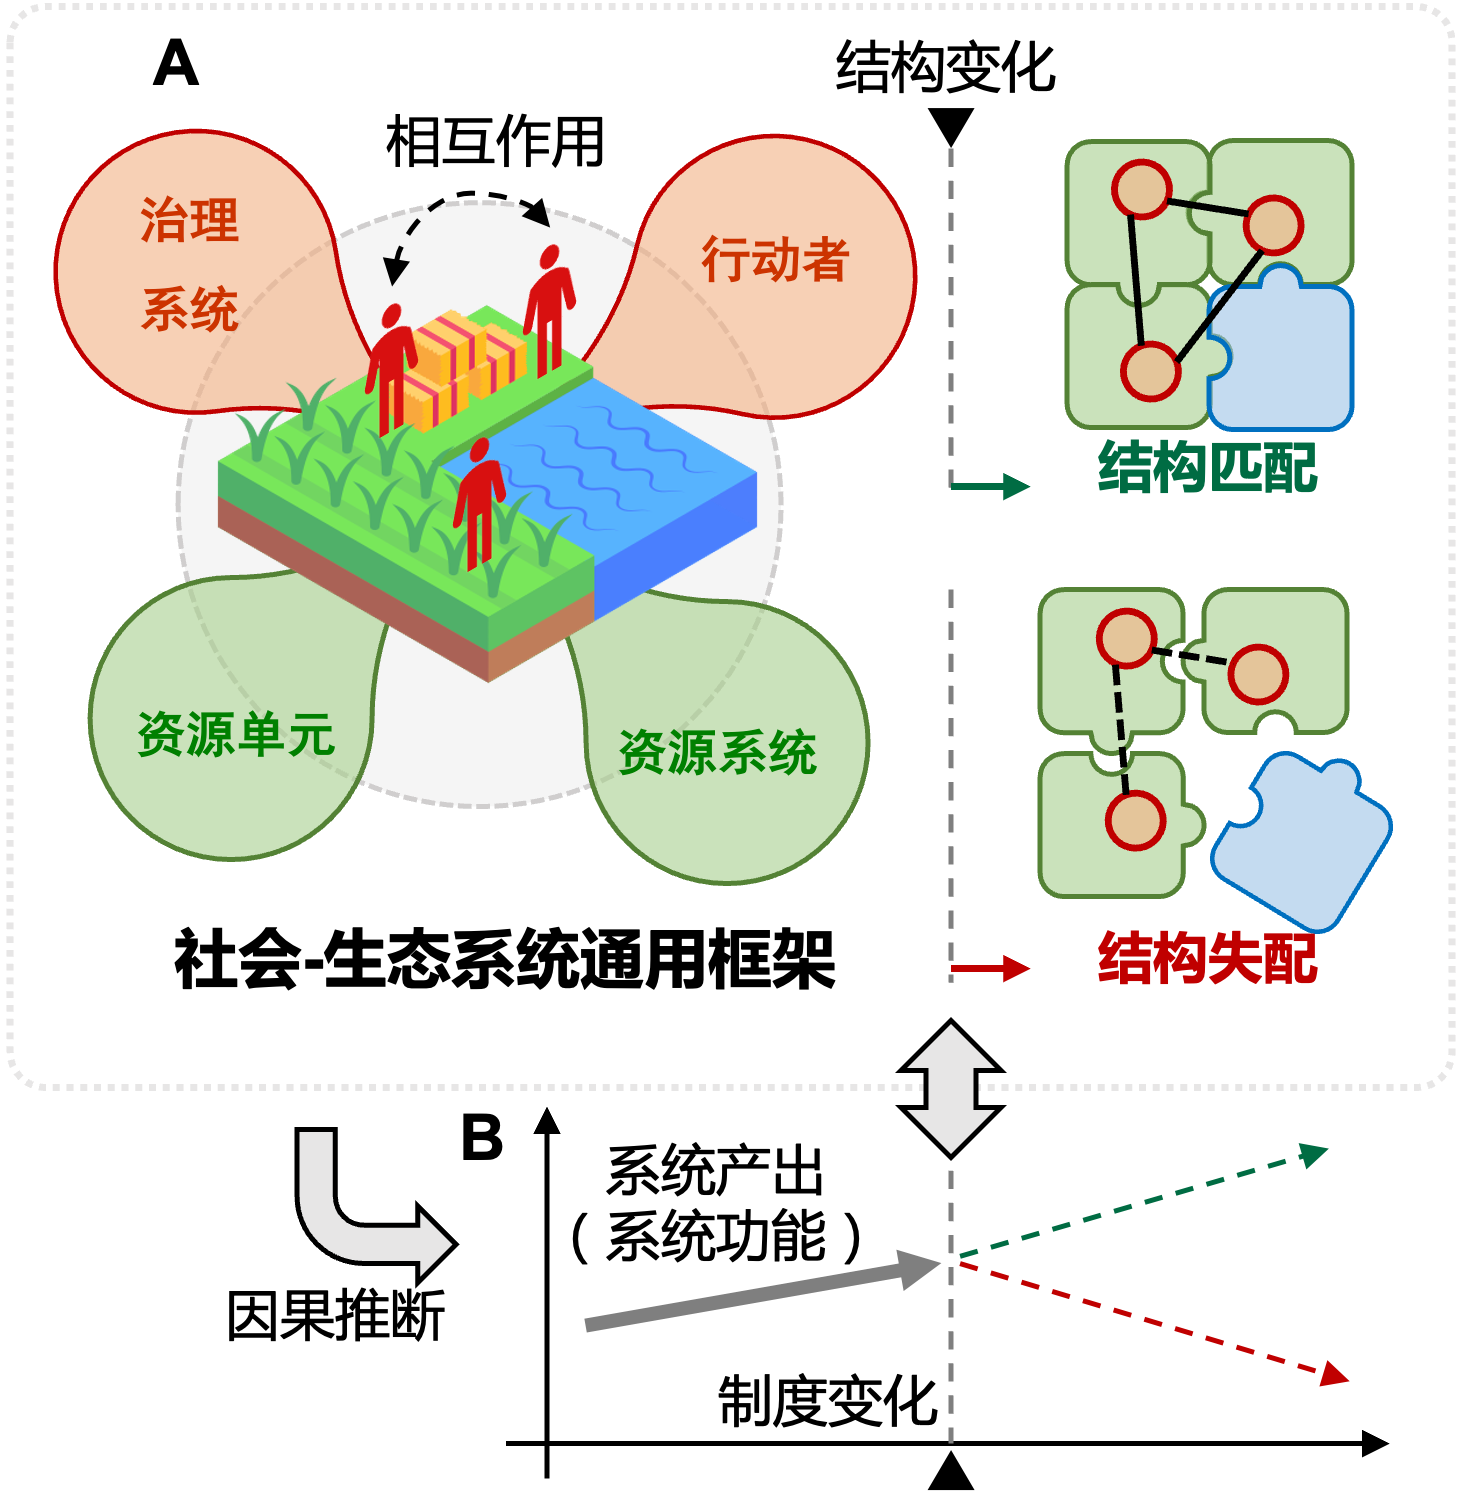
\includegraphics[width=0.6\textwidth]{img/ch5/ch5_framework.png}
    \caption[社会-生态系统结构和结果之间的因果推断框架]{社会-生态系统结构和结果之间的因果推断框架。\textbf{a.}分析社会-生态系统的通用框架(改编自 Ostrom, 2009~\cite{ostrom2009})内,制度改革可以通过改变系统内部的相互作用重塑结构。\textbf{b.}通过构建反事实推断,可以分析匹配/不匹配SES结构如何影响系统演变。}\label{fig:framework}
\end{figure}

\subsection{数据与预处理}\label{sec:dataset}

为构建反事实推断模型,需要选择表征实际用水情况的因变量,以及能够用以预测地区用水量的自变量。
本章研究从国家水利部开展的用水量调查数据作为观测值,从不同来源获取了农业、工业、服务业、居民生活、环境五个类别共计$24$个影响区域用水的社会、经济、环境因素作为自变量\cite{zhou2020}(见表~\ref{ch5:tab:data_source})。
数据集的空间范围包括中国$30$个省、自治区、直辖市和地区(不包括台湾、香港、澳门;天津和河北因在分水政策中被合在一起考虑,因此合并两地数据为“津冀”)。
数据集的时间范围涵盖两次政策前后各十年,即$1979$年至$2008$年,数据所有特征在该时间段内均无任何缺失值。

% Table generated by Excel2LaTeX from sheet '数据来源'
\begin{table}[htbp]
    \caption{推断地区用水量的自变量数据}
      \begin{tabularx}{\textwidth}{LLLL}
      \toprule
      \multicolumn{1}{l}{部门} & 分类    & 单位    & 描述 \\
      \midrule
      \multicolumn{1}{l}{农业$^1$} & 灌溉面积  & 千公顷   & 装配了灌溉设施的不同作物面积 \\
      \multicolumn{1}{l}{工业$^2$} & 产值    & 千百万元  & 工业各产业的总增加值 \\
            & 循环用水比例 & \%    & 工业循环用水占总用水比例 \\
      \multicolumn{1}{l}{服务业} & 服务业总增加值 & 百万元   & 服务业的总增加值 \\
      \multicolumn{1}{l}{居民生活} & 城市人口  & 百万人   &  \\
            & 农村人口  & 百万人   &  \\
            & 牲畜数量  & 十亿千焦  & 牲畜卡路里总和 \\
      \multicolumn{1}{l}{环境} & 气温    & K     & 近地表气温 \\
            & 降水量   & mm    & 年累计降水量 \\
      \bottomrule
      \end{tabularx}\label{ch5:tab:data_source}%
      \footnotesize
      1. 包括以下作物类型:水稻、小麦、玉米、水果、其它
      2. 包括以下产业:纺织、造纸、石油化工、冶金、采矿、粮食生产、水泥、机械、电子、电力、其它
\end{table}%
  

在“八七”分水方案和流域统一调度均涉及的$10$个省份或地区中,四川、津冀因为从黄河流域取用水占该地区总用水量不足$5\%$而不作为“受政策影响区域”,被剔除(见表~\ref{ch5:tab:quota})。
由于数据的量级和单位相差较大,为便于后续研究,在进行分析前统一对数据集的所有特征进行标准化(见式\ref{ch5:eq:normalization})。
\begin{equation}
    x_{\textit{normalized}}=\frac{x-\bar{x}}{s}
    \label{ch5:eq:normalization}
\end{equation}
其中,$x_i$ 表示第 $i$ 个数据,$\bar{x}$ 表示数据的均值,$s$ 表示标准差。

此外,分水制度的提出与实施直接原因是解决黄河$1970s$年以来的断流问题\cite{wang2019b},本文还使用了研究时段内的黄河断流数据(包括断流的天数和河段长度)和流域的平均干旱指数数据\cite{wang2022e}。

\subsection{主成分分析}

主成分分析(Principal Components Analysis, PCA)是一种用于降低大型数据集维度的技术。PCA 利用原始变量的线性组合创建了一个新的变量集,这些新的变量被称为主成分(PC)。
Bayan(2021)\cite{bayani2021}已证明了将PCA与合成控制法(Synth Control, SC)相结合可以提高其因果推理的鲁棒性。
面板数据不能直接应用 PCA,本章研究将所有预处理后的数据沿时间轴进行多年平均,对均值使用主成分分析(PCA)进行降维,将得到的主成分按照其在原始数据中解释方差变化的大小顺序进行排序,并用肘部法确定主成分的个数,从而降低反事实推断合成控制模型的自由度。

负荷率代表每个原始变量与主成分之间的相关性,通过原始变量在每个主成分上的负荷,可以分析对区域用水量贡献最大的主成分与特征集合有关,了解用水量影响特征与主成分的相互关系。
参考 Mirco 等人(2021)的研究,每个特征对于特定主成分的贡献是否显著主要有三种方法:特征向量法、负荷阈值法、固定阈值法~\cite{migliavacca2021}。
本章研究采用负荷阈值法分析各特征对不同主成分的贡献,即当负荷值的绝对值和贡献大于与维数(即变量)相关的特定阈值时(即$|{x_{loading}}| > 1/N_{dims}$),认为该特征对当前主成分的贡献显著。


\subsection{差分合成控制法}\label{sec:DSC}

本章研究选用差分合成控制法(Differenced Synthetic Control, DSC)构建反事实推断模型,估算不受制度改革影响情景下的流域用水量,从而对分水制度的影响进行因果推断(Causal Inference)。
DSC 方法是对合成控制法(Synthetic Control, SC)在鲁棒性上的改进\cite{billmeier2013, smith2015},这一类因果推断方法可以构建一个可比的控制单元来估计历史事件或政策干预对真实单元(如城市、地区和国家)的影响及其变化趋势\cite{abadie2010, abadie2015, hill2021}。
将经降维处理的数据集分为反事实推断所需的“实验组”和“对照组”数据,其中水配额制度涉及的省份数据作为目标组$(n=8)$数据,其他省份则作为对照组$(n=20)$数据。
该方法旨在评估政策变化的影响,而这些政策变化集中在其中一些单元上,在本研究中即为分水制度涉及的省份属于政策影响的单元,称之为“处理单元”,其用水特征作为“真实值”使用“目标组”数据的因变量进行表达。
合成控制法通过重新加权非处理单元构造其凸组合作为控制组,并匹配处理单元和控制单元在政策干预前的变化趋势构成反事实推断,这一来处理单元和控制单元在政策干预后的因变量差异便可估计为政策干预的净效应。

本章研究中,所有处理单元(即制度涉及的诸省)都在1987年和1998年先后受到两次不同的制度干预,因此每个政策干预前后十年都被视为单独的分析时期,即一次构建反事实推断模型的研究时段可能为 $1979 \sim 1998$(1987年为政策干预时点)或 $1987 \sim 2008$(1998年为政策干预时点)。
接下来将黄河流域分水制度涉及的每个省份分别作为处理单元($n=8$,见\textbf{\nameref{sec:dataset}}),其余的$J=20$个控制单元均来自流域外未受“政策干预”的省份构建模型,而这种多处理单元的合成控制法也已广泛应用\cite{abadie2021}。
% 然后,我们认为在第$T = {1,2 \ldots , T}$时间段观测到的第$J+1$个单位。
我们定义$T_0$为政策干预前的周期数(年份,$1,\ldots,t_0$),定义$T_1$为政策干预后的周期数($t_0,\ldots,T$),使得$T = T_0+ T_1$,每个处理单元在政策干预后的时间$T_1$内都面临制度变迁,而在之前的$T_0$时期不受政策干预的影响。
这一来,控制单元的任何加权组合都是一个潜在的合成控制模型,可以用一个权重为$\mathbf{W} = (w_{1},\ldots,w_{J}), w_j \in (0, 1)$的向量$J * 1$来表示。
通过引入$k * k$的对角线半定矩阵$\mathbf{V}$表示各协变量相对重要性,那么在所有潜在合成控制模型中求解最优合成控制权重$W$的过程为:

\begin{equation}
    \mathbf{W^{*}(V)}=\underset{\mathbf{W} \in \mathcal{W}}{\operatorname{minimize}}{\left(\mathbf{X}_{\mathbf{1}}-\mathbf{X}_{\mathbf{0}} \mathbf{W}\right)}^{\prime} {\mathbf{V}}{\left(\mathbf{X}_{\mathbf{1}}-\mathbf{X}_{\mathbf{0}} \mathbf{W}\right)}
\end{equation}

给定$\mathbf{V}$的情况下,$\mathbf{W}$是矩阵$\mathbf{W}^{*}(V)$的权重向量,使处理单元与控制单元之间的特征差异最小。
这意味着$\mathbf{W^{*}}$取决于对$\mathbf{V}$的选择,因此可以用$\mathbf{W*(V)}$表示。
差分合成控制法选择$\mathbf{V^{*}}$作为优化$\mathbf{W*(V)}$的$\mathbf{V}$,通过让政策干预单元和合成控制法构建的对照单元在政策干预前的结果差异最小化:

\begin{equation}
    \mathbf{V}^{*}=\underset{\mathbf{V} \in \mathcal{V}}{\operatorname{argmin}}{\left(\mathbf{Z}_{1}-\mathbf{Z}_{0} \mathbf{W}^{}(\mathbf{V})\right)}^{\prime}{\left(\mathbf{Z}_{1}-\mathbf{Z}_{0} \mathbf{W}^{*}(\mathbf{V})\right)}
\end{equation}

其中$\mathbf{Z}_{1}$是一个$1*T_0$的矩阵,包含政策干预单元在干预前的每一个观察样本。
类似地,让$\mathbf{Z}_{0}$作为一个$k * T_0$的矩阵,其中包含了政策干预前期控制单元每个的观察结果,其中$k$为数据集中变量的数目。

\subsection{结果鲁棒性检验}

对合成控制法(DSC)的鲁棒性测试方法主要有两种。
首先,可以比较处理前后(此章研究中为流域分水政策的干预)对推断变量(此章研究中为用水量)的重建效果,如在处理前重建的模型预测值与实际观测值差距很小,重建后的预测值和观测值差距很大,则说明政策干预的效果非常明显。
本章研究中,为判断干预效果是否显著,使用配对样本$T$检验计算统计量,针对1987年“八七”分水方案1998年流域统一调度两次制度干预,分别对其制度干预前期、后期的模型预测和实际观测数据进行检验。
若政策干预后的 $p-value$ 小于阈值(本章研究采用置信度水平95\%即阈值为$0.05$),则能够拒绝“两者无显著差异”的原假设$H_0$,认为制度干预让该区域用水量发生了显著变化。
若与此同时,制度干预前$T$检验的显著性水平大于阈值,则说明DSC模型在制度干预前成功预测了该地区用水量随时间的变化,拟合效果很好。

其次,安慰剂试验是评估合成控制方法有效性的另一种常见方式。
在安慰剂试验中,用一个从控制单位库中选出的安慰剂单位代替被处理单位,然后使用与被处理单位相同的数据和参数,对安慰剂单位实施合成控制方法。
如果合成控制方法是有效的,它应该在安慰剂单位和控制单位之间产生明显的差异,因为安慰剂单位不应该受到干预的影响。
安慰剂测试可以用来评估合成控制方法的有效性,并检测分析中的任何偏差或混杂因素。
我们采用 Abadie(2010)年提出合成控制法时建议的安慰剂检验步骤\cite{abadie2010},使用 Dmitry 等人提出的差分合成控制法的 Python 库进行安慰剂检验,如果在大多数省份中,合成后期均方根误差(MSPE,见式\ref{ch5:eq:RMSE})与合成前期的比率显著高于(同样采用$T$检验判断差异的显著性)其他安慰剂单位的结果,则表明在制度处理时期(此处为1987年和1998年)黄河流域受影响比大多数其他省份影响更大。

\begin{equation}
    \label{ch5:eq:RMSE}
    \text{RMSE} = \sqrt{\frac{1}{n}\sum_{i=1}^{n}{(y_i-\hat{y}_i)}^2} 
\end{equation}

其中$n$为观测数,$y_i$为实际值,$\hat{y}_i$为预测值。

\subsection{计算方法与软件实现}

主成分分析使用了$pca$软件包(v-1.9.1)\cite{Taskesen_pca_A_Python_2020},单差分合成控制法在其作者公开的$Synthetic Control Methods$软件包基础上修改完善\cite{arkhangelsky2021}。所有库在 Python 3.11.2 环境下运行,本章研究的所有代码已公开在GitHub\cite{song2022c}。
